\documentclass[11pt, twoside, reqno]{article}
\usepackage{amssymb, amsthm, amsmath, amsfonts}
\usepackage{graphicx}
\usepackage{color}
\usepackage{hyperref}
\usepackage{verbatim}
\usepackage[toc,page]{appendix}
\usepackage{listings}
\usepackage{chngpage}
\usepackage{float}
\usepackage[shortlabels]{enumitem}
\usepackage{csvsimple}
\setlist[enumerate, 1]{1\textsuperscript{o}}

\definecolor{codegreen}{rgb}{0,0.6,0}
\definecolor{codegray}{rgb}{0.5,0.5,0.5}
\definecolor{codepurple}{rgb}{0.58,0,0.82}
\definecolor{backcolour}{rgb}{0.95,0.95,0.92}

\lstdefinestyle{mystyle}{
    backgroundcolor=\color{backcolour},
    commentstyle=\color{codegreen},
    keywordstyle=\color{magenta},
    numberstyle=\tiny\color{codegray},
    stringstyle=\color{codepurple},
    basicstyle=\footnotesize,
    breakatwhitespace=false,
    breaklines=true,
    captionpos=b,
    keepspaces=true,
    numbers=left,
    numbersep=5pt,
    showspaces=false,
    showstringspaces=false,
    showtabs=false,
    tabsize=2
}

\lstset{style=mystyle}

\begin{document}

\section{Introduction}
\hspace{0.2in}At the end of Chapter \ref{ch:3} we discussed building sentiment profiles for a candidate. These profiles are inspired by the profiles that many polling places create as they ask questions on their candidate. To run with the inspiration, this chapter dives into the dataset that we've created and examines if trends found in polling are reflected on twitter.  

\section{Races Collected}
\hspace{0.2in}In the data gathering process, tweets were collected from thirty-three senate races, twenty nine house races, and a series of miscellaneous hashtags designed to capture national sentiment about the election. 

After counting tweets and more, displayed below are leaderboards for house and senate. The most popular races consisted of the races with the most tweets. The Most Tweets category refers to the candidates that were tweeted about the most. The Best Liked goes to the candidate that had the highest portion of positive tweets. Least liked and Most Neutral work the same way, except for Negative and Neutral tweets respectively. There was a five hundred tweet minimum to qualify for the leaderboard. 
\begin{center}
\begin{tabular}{ |c|c|c|c|c|c|} 
	\hline
	Rank & Most Popular Race & Most Tweets & Best Liked & Least Liked & Most Neutral \\
 	\hline 
	1 & Texas Senate & Ted Cruz & Angela Green & Josh Hawley & Tony Campbell\\
  	\hline
	2 & Florida Senate & Rick Scott & Lawrence Zupan & Angus King & Kevin Cramer\\ 
	\hline
	3 & Indiana Senate & John James & John Barasso & Bill Nelson& Matt Rosendale\\
	\hline
\end{tabular}
\end{center}
\begin{center}
\begin{tabular}{ |c|c|c|c|c|c|} 
	\hline
	Rank & Most Popular Race & Most Tweets & Best Liked & Least Liked & Most Neutral \\
 	\hline 
	1 & NY-22 & Troy Balderson & Xochitl Small & Josh Hawley & Lizzie Fletcher\\
  	\hline
	2 & VA-07 & Steve Knight & Harley Rouda & Angus King & John Culberson\\ 
	\hline
	3 & KY-06 & Mike Bishop & Ross Spano & Bill Nelson& Gil Cisneros\\
	\hline
\end{tabular}
\end{center}
%Aggregate sentiment score vs the percentage of tweets that are positive 
%The 

One interesting point is that those who lead the various sentiment-based categories were no where close to the leaderboard in the most tweets category. Generally it felt that if a candidate was tweeted about more, their average sentiment score tended to drift towards neutral with the positive and negative tweets balancing out. Here is that relationship in graph form. 
\begin{figure}[H]
\centering
	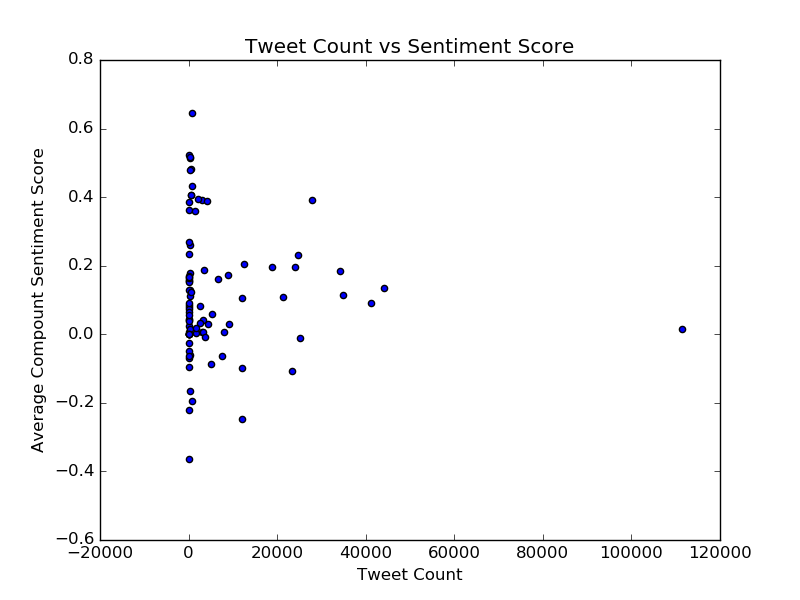
\includegraphics[scale=0.5]{count_sentiment}
\end{figure}

%More content. Exact numbers on people that fall into those ranges
%Standard deviation of the groups - speak on exact terms. Larger standard deviation in the group with smaller tweets. 
%Make the bins smaller and plot the standard deviation
%Address that the most neutral board is made of the percentage of neutral tweets

%Lets look at the count because it's a 

As the count increases, the range in sentiment scores decrease. The samples with tweet counts greater than twenty thousand all stay within a range of 0.4 on either side of neutral. Conversely, the range for sample sizes less than twenty thousand is from -0.4 all the way to 0.7. Essentially, the larger sample sizes are more balanced with a number of positive and negative tweets. That lends support to the idea that our sample isn't overly biased in one ideological direction. 
\section{Comparing Sentiment}

\subsection{Winners vs Losers}
\hspace{0.2in}The point of an election is to win. The question everyone wants to answer is how? What's separates the winners from the losers, and how is that reflected on Twitter? Let's take a look at all the features from the sentiment profiles we created in Chapter \ref{ch:3}. We'll begin with the senate. 

The graph below shows the average compound sentiment score for winning and losing Senate candidates.
\begin{figure}[H]
\centering
	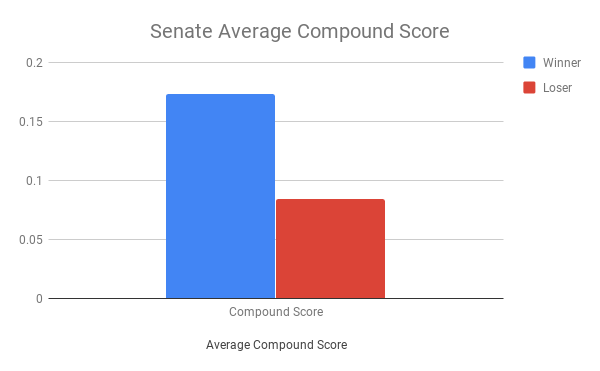
\includegraphics[scale=0.5]{sen_ave_score}
\end{figure}
The winning candidates are heads and shoulders above the losing candidate, and have a much better sentiment score as a whole. That feels right. Candidates that win elections are favored by the voters and that should be reflected on twitter. 

Compound score is a combination of positive and negative tweets. If winners have a higher compound score, it stands to reason that losers will have more negative tweets than winners. The next figure breaks down the count by type of tweet - positive/negative/neutral. 

\begin{figure}[H]
\centering
	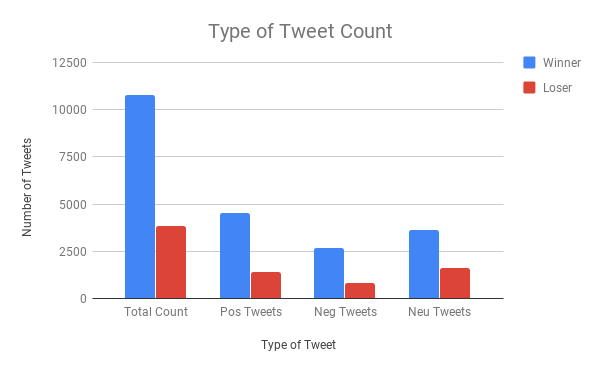
\includegraphics[scale=0.5]{tweet_type}
\end{figure}

The election losers don't actually have fewer negative tweets. That's probably because there's just so many more tweets regarding winners than there are losers. To get a better view, let's break down types of tweets into percentages of the total count. That is to say, what percentage of a winner's tweets are positive, negative, or neutral?

\begin{figure}[H]
\centering
	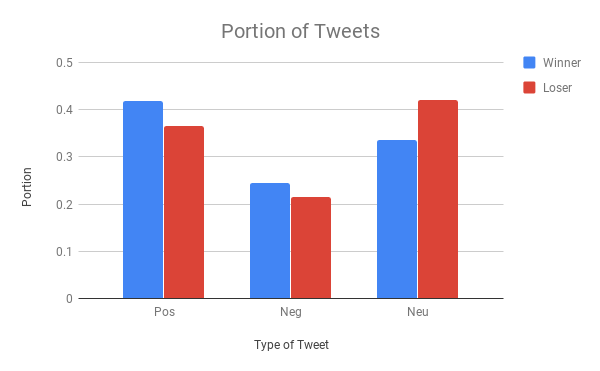
\includegraphics[scale=0.5]{tweet_breakdown}	
\end{figure}

A closer look shows that the real difference lies in the fact that losers have a greater portion of neutral tweets than winners do. In therms of positive and negative tweets, the portions differ by less than five percentage points. Neutral tweets have a sentiment score of zero which would dilute and lower the average compound scores. Winners are not only tweeted about more than losers, but they're more likely to have tweets that show \textit{some} sentiment. But do these patterns hold true for the house?

The average compound scores for winners and losers are displayed below:

\begin{figure}[H]
\centering
	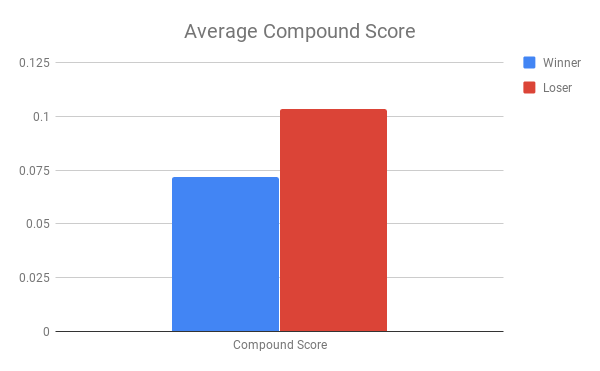
\includegraphics[scale=0.5]{house_compound}
\end{figure}

Unlike the senate, the losers had a higher average sentiment score than the winners. That's unexpected. Let's take a deeper look into how those numbers break down. 

\begin{figure}[H]
\centering
	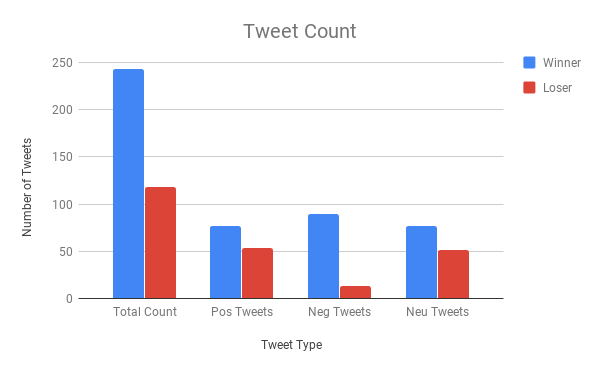
\includegraphics[scale=0.5]{house_tweet_type}
\end{figure}

Winners do have more positive tweets, but the large difference in the number of negative tweets is what ultimately influences the lower average compound score seen. Unlike the senate, the house races show an even-ness when it comes to neutral tweets. These numbers are hardly conclusive, partially because the large difference in tweet count is inflating these numbers. Here's a breakdown of the tweet portions:

\begin{figure}[H]
\centering
	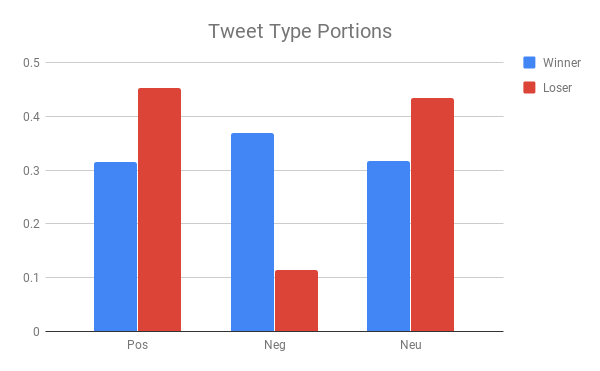
\includegraphics[scale=0.5]{house_tweet_breakdown}
\end{figure}

The house and the senate winners both roughly have 30\% of their tweets designated neutral. The real difference is that negative tweets occupy a far higher proportion of tweets. It doesn't feel that positive and negative tweets have a distinguishable effect on winning. In fact, the only trend that holds across both house and senate winners is the fact that winners are just tweeted about more. The house had a ratio of about 2-to-1 while the senate had 3-to-1. Bottom line, positive tweets are preferred, but overall engagement is key. 

\subsection{Democrats vs Republicans}
The two party system is a large part of our election process. The parties command massive influence and many voters choose a candidate based entirely on party affiliation. This means that a party's national platform and performance can influence their performance in more local elections like the house and the senate. 

In the house, the Democrats flipped a number of Republican Incumbents taking a majority. In the Senate, the Republicans held the majority thanks to the uneven split in seats up for election.

\begin{center}
\begin{tabular}{|c|c|c|}
	\hline
	Incumbents & House & Senate \\
	\hline
	Democrats & 1 & 24\\
	\hline
	Republicans & 28 & 9\\
	\hline
\end{tabular}
\end{center}

\begin{center}
\begin{tabular}{|c|c|c|}
	\hline
	Winners & House & Senate \\
	\hline
	Democrats &  &  \\
	\hline
	Republicans &  &  \\
	\hline
\end{tabular}
\end{center}

In the previous section, it showed that overall sentiment and tweet counts were two features that winners of elections had. If those traits hold, it should show that Democrats in the house should have a higher average sentiment and more tweets and the same for Republicans in the Senate. 

\begin{figure}[H]
\centering
	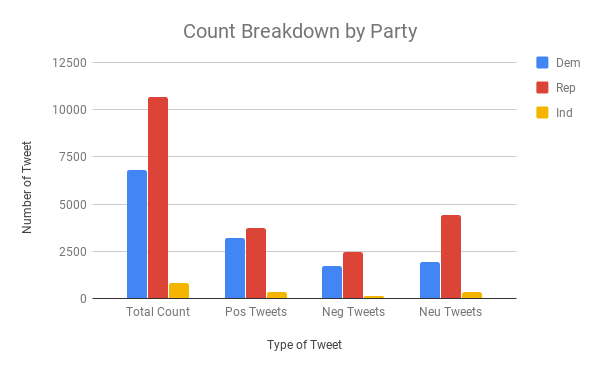
\includegraphics[scale=0.5]{count_party_senate}	
\end{figure}

The Republican dominated Senate did indeed carry the higher total count. They also led in every single other category. This will have interesting effects on the actual sentiment comparison.

\begin{figure}[H]
\centering
	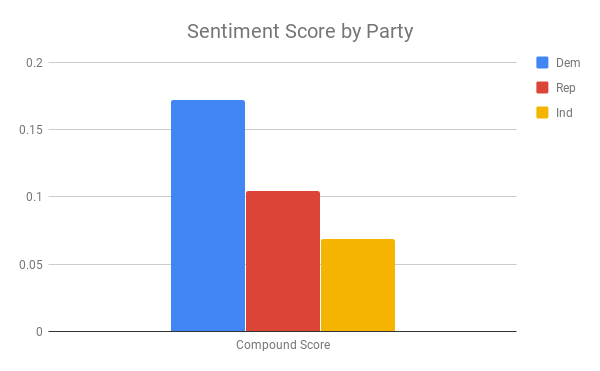
\includegraphics[scale=0.5]{party_sent}
\end{figure}

Republicans leading both in positive and negative tweets meant that they suffered in the overall sentiment tally. The winning party held the tweet count lead, but not overall sentiment. If tweet count is truly the major feature to follow, the trend should hold in the house.

\begin{figure}[H]
	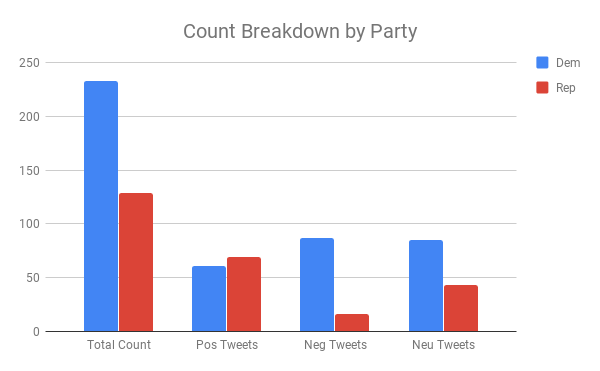
\includegraphics[scale=0.5]{count_party_house}
\end{figure}

\begin{figure}[H]
	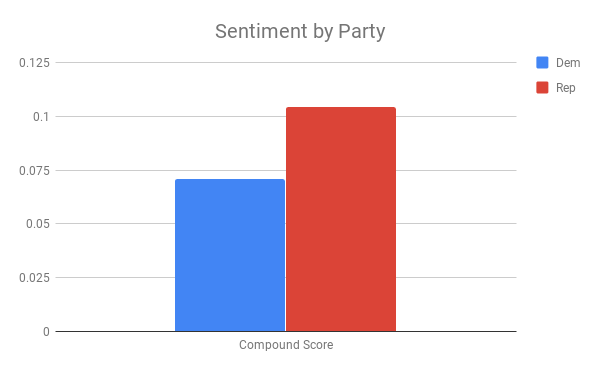
\includegraphics[scale=0.5]{party_sent_house}
\end{figure}

The main takeaway here is that the tweet count lead continues to hold. The sentiment score favors the Republicans - the losing party - but that correlates with the fact that losing candidates in the house had a better sentiment score as well. 

\section{National Trends}
\hspace{0.2in} This data set presents the opportunity to explore how national trends are reflected on twitter. Not only that, it'll give a better idea on the kind of sample collected and how it reflects to the samples pollsters take when they observe overall trends they expect to influence elections. 

Eight search terms were used to create a database of miscellaneous tweets. These search terms were largely national trends:

\begin{figure}[H]
	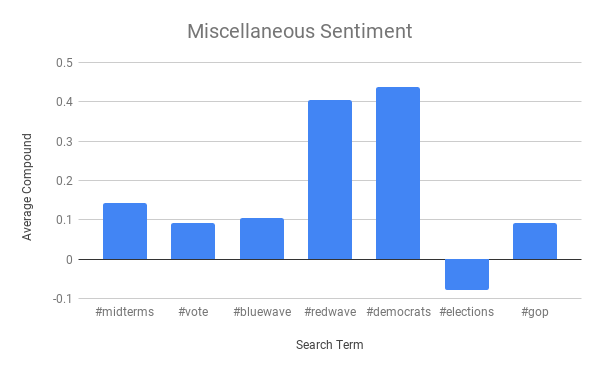
\includegraphics[scale=0.5]{misc_sent}
\end{figure}

The sentiment of partisan search terms are about the same. Non-partisan terms have sentiments within a similar range with the peculiar exception of ``\#elections". The purpose of this exercise was to show that this database is mostly neutral in contrast to the house leaning democrat and the senate republican. 

The three major trends we're examining are sourced from an ABC news article published on November 6th. The article identified health care, border security, and Donald Trump as three major factors heading into the midterm election.

\subsection{Exploring the Issues}
\label{subsec:exploring the issues}
\hspace{0.2in}The main motivation for this project \textit{was} Donald Trump. Mr. Trump was a controversial candidate and is now a controversial president. The midterms are often considered a referendum against the president. Areas which view Mr. Trump favorably should lean republican while those who don't favor him should lean democrat. Since taking office, Mr. Trump has averaged a favorability rating of forty percent while never being higher than forty-five. 

Health care has had an interesting history in US Politics. In 2010, President Barack Obama passed the Affordable Care Act allowing access for millions of uninsured. Despite many Republican efforts, including a late push by congress in 2018, the ACA still stands. Several moderate Republicans avoided voting against it due to its popularity in their district/state. 

According to the Kaiser Family Foundation, the ACA continues to remain a hot topic among voters. A different Pew Research poll showed that sixty percent of voters believe that health care is the government's responsibility. 

The last major issue is the border wall. Mr. Trump's first campaign promise was the wall and his continued attacks on illegal immigration gained him significant support. After taking office, Mr. Trump has wielded the Immigrations and Customs Enforcement Division (ICE pronounced "ice") as a baton to round up and deport illegal immigrants. A gallup poll had just twenty percent of respondents view Illegal Immigration as ``not a problem". 

These three issues are front and center, and the data set should have views about them. Having Twitter's numbers agree in some form with that of traditional pollsters shows that the data set is a fair representation of the populace. 

\subsection{Evaluating Twitter's Response}
\hspace{0.2in}There were six search terms taken from the three issues. Using modified code that can be found in Appendix B, a sentiment profile was put together. Each term was searched independently in the senate, house, and miscellaneous database. The goal was to have the three databases capture a different type of population. 
\begin{figure}[H]
	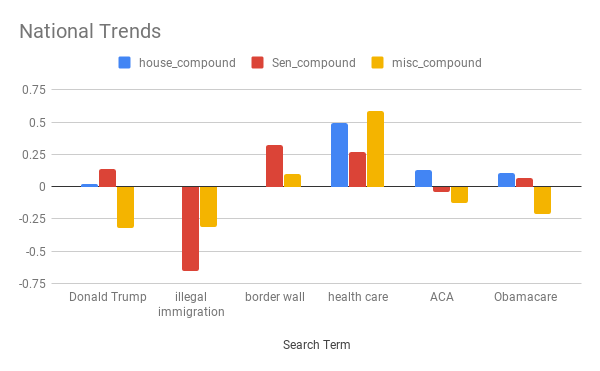
\includegraphics[scale=0.65]{natty_trends}	
	\caption{Sentiment scores of search terms that describe important national trends}
	\label{fig:natty_trends}
\end{figure}

Looking at Figure \ref{fig:natty_trends} that assumption holds up. Mr. Trump is viewed favorably in the Republican dominated Senate, while less so in the house and in general. His house sentiment may be a result of a majority of house elections had republican incumbents. His intense negative sentiment with the general populace correlates with that of his general favorability - which is below average. 

On illegal immigration, it's interesting to see that Democrats took no stance. That could be because if they did, they would be in the minority. Sentiment is decidedly against illegal immigration and very much for the border wall. This is not only in the republican-dominated Senate but in the more neutral miscellaneous database. It's possible that Democrats saw a path through success by simply not addressing illegal immigration and focusing on other topics that were in their favor like health care. 

In section \ref{subsec:exploring the issues} a Pew research poll was referenced regarding health care and the government. Specifically voters believed that health care was a governmental responsibility. They've echoed that sentiment here, as big fans of health care as an idea in general, but not of specifically the ACA. Notice that the ACA and Obamacare reference the same piece of legislation, but Obamacare's sentiment is noticeably lower in all three categories. That may be because of the vitriol Obama faces by Republicans and even the nation. It's clear that Obama's controversial presidency is still showing effects. So much so, that just the name on the paper makes all the difference.  

\end{document}

